% The chapter presents an overview of the architecture of CacheInf.

\subsection{Working Environment}
We assume that the working environment of CacheInf is a mobile robot performing robotic tasks in the real world which requires seamless real-time visual model inference on the continuous image stream captured from the on-board camera, to achieve real-time response to various environment changes.
The robot itself is equipped with low-power-consumption gpu to perform slow and comparatively high energy consumption local visual model inference so as to guarantee its worst case performance; it has wireless network access to a remote powerful GPU server that provides opportunities of acceleration via computation offloading, but the connection suffers from limited and unstable wireless network bandwidth.

% While the requirements of real-time inference does not necessarily imply the requirement of high inference frequency, we measure the real-time metric by the average end-to-end inference latency when the robot is seamlessly performing inference, which leads to high inference frequency; the power consumption is also measured by average power consumption to finish inference on each image in the same scenario.

\begin{figure*}[!htb]
    \centering
    %\vspace{-0.2cm}
    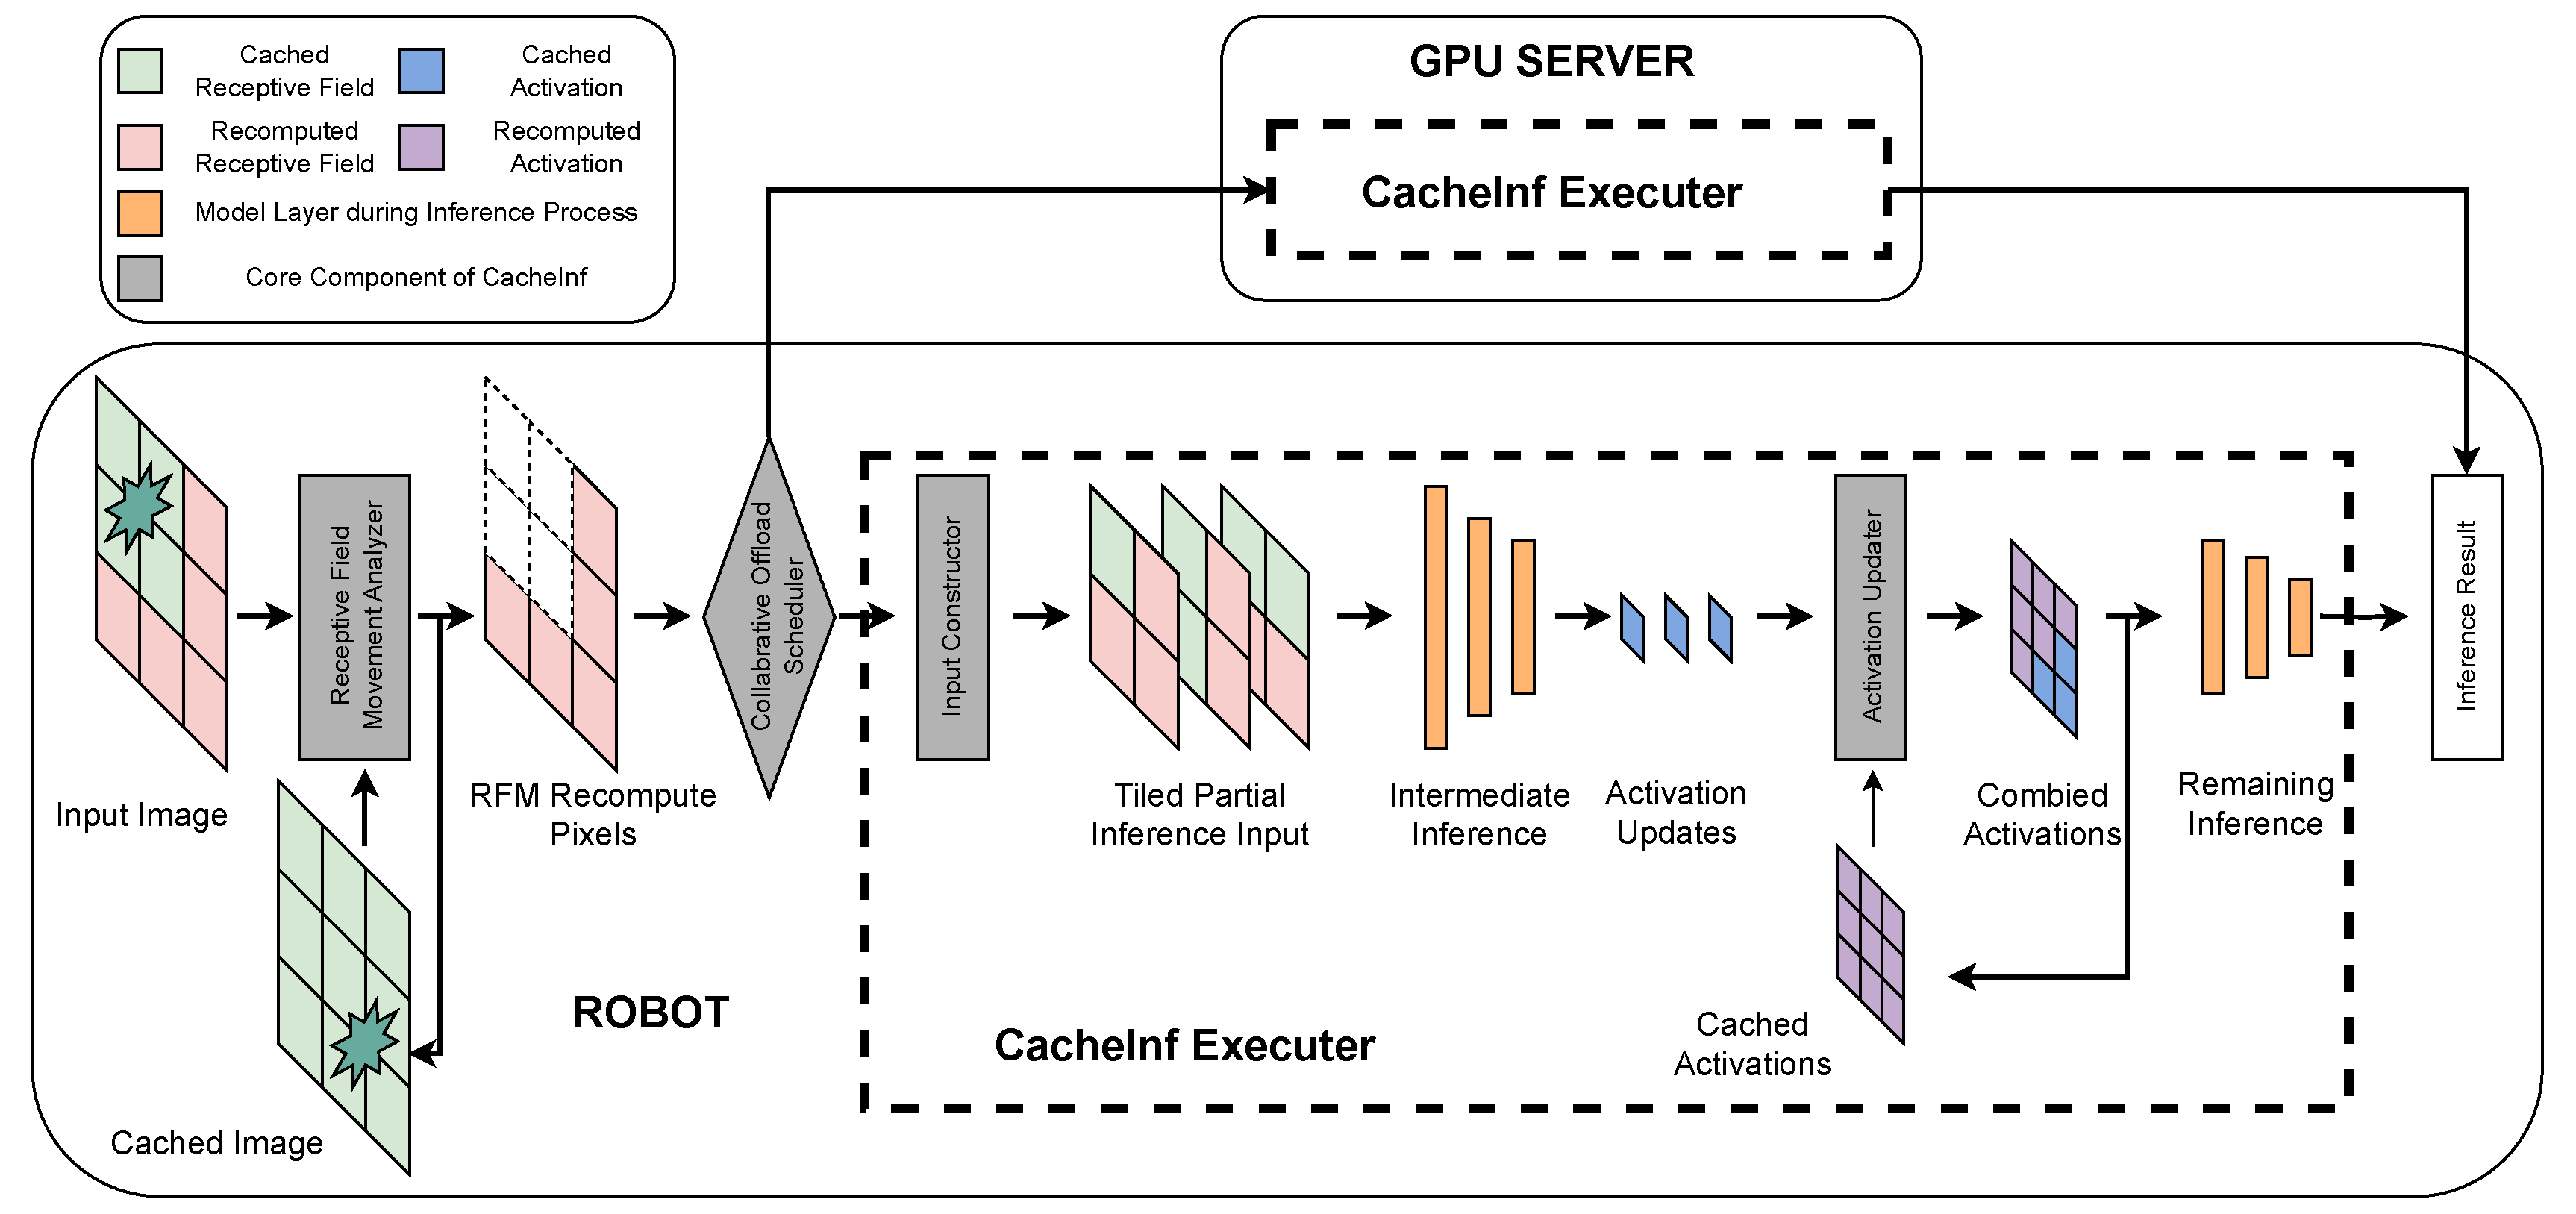
\includegraphics[width=\linewidth]{fig/overview_new_new.drawio.pdf}
    %\vspace{-0.2cm}
    \caption[track]{Architecture and workflow of CacheInf. }
    \label{fig:overview}
    %\vspace{-0.3cm}
\end{figure*}


\subsection{Architecture of CacheInf}
CacheInf consists of four major components: Collaborative Offload Scheduler, Cache Analyzer, Cache Combiner, and Recomputation Input Constructor.
Figure~\ref{fig:overview} describes the runtime workflow of CacheInf.
Collaborative Offload Scheduler functions both at the initialization stage and at runtime and we exclude the initialization stage in Figure~\ref{fig:overview} for simplicity.
For simplicity, we call the Recomputation Input Constructor and Cache Combiner for activations together with the visual model inference pipeline as the CacheInf Executor which resides on both the robot and the GPU server.

\subsubsection{Collaborative Offload Scheduler}
During the initialization stage of the robotic task and CacheInf is granted access to a visual model and an initial input image.
Collaborative Offload Scheduler first profiles the visual model based on this initial input and its execution statistics (e.g., execution time of each operator and the receptive field) on both the robot and the server.
Then it finds the operator involved in the visual model that should cache its computation results (activations) and computes for an optimized computation and offloading plan for each possible situation including different wireless network bandwidth and different ratios of recomputation.
To operator to cache its computation results is typically the last operator that preserves the spatial information of the input images (i.e., convolution, pooling, element-wise addition/subtraction, etc), which is typically the operator before operators such as flatten and matrix multiplication.

At runtime Collaborative Offload Scheduler collects the running statistics such as wireless network bandwidth and the ratio of recomputation and at a fixed interval (e.g., several inference) rearrange the placement of computation (either locally compute or offload the computation to the GPU server) according to the precomputed schedule accordingly for optimal inference acceleration.
The rearrangement can also be triggered when extreme conditions are detected, such as almost zero wireless network bandwidth or a full recomputation on the input image is required.


\subsubsection{Cache Analyzer}
\begin{figure}
    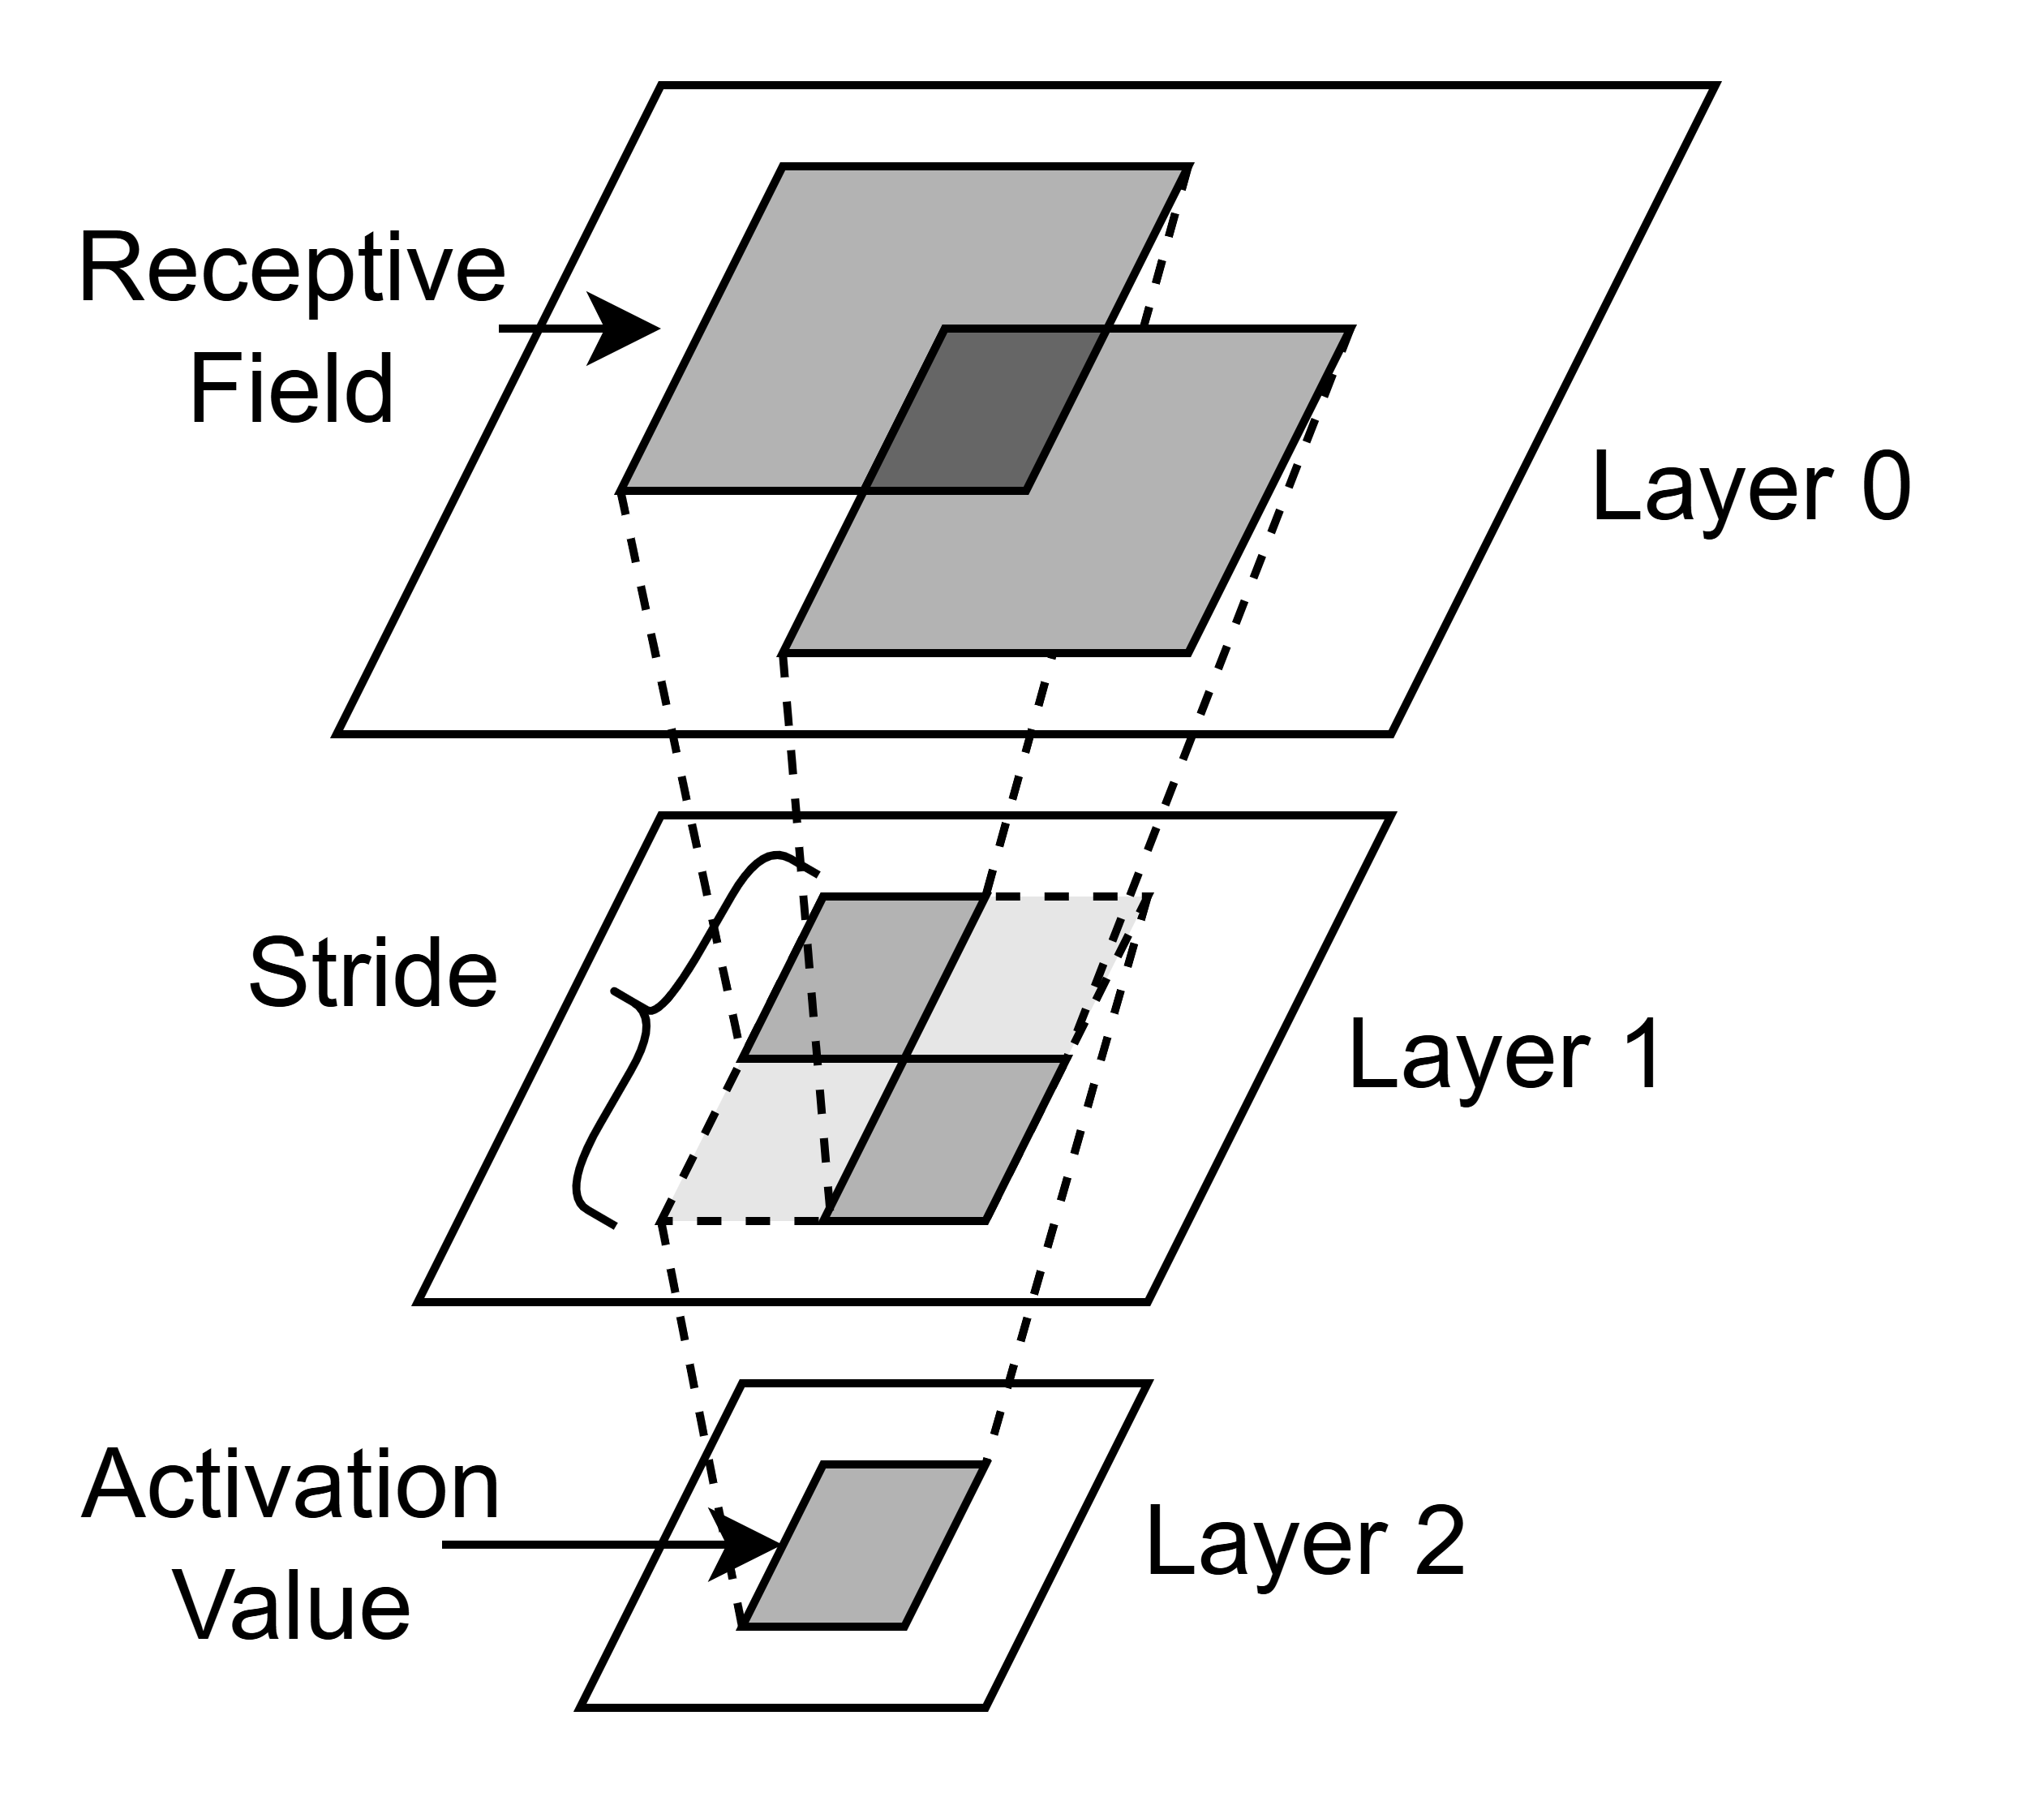
\includegraphics[width=0.5\linewidth]{fig/insight.drawio.png}
    \caption[short]{Receptive fields and their dominated pixels on the activations.}
    \label{fig:receptive field}
\end{figure}
Given a new input image, Cache Analyzer contrast it with the cached input image to find the movements of the receptive fields of the cached activations.
Since the receptive fields of different pixels on the activations often overlaps as shown in Fig.~\ref{fig:receptive field}, we first divide the whole input image into different small pixel blocks and calculate the movements of each pixel blocks (represented by motion vectors) via pixel block matching.
The movements of the pixel blocks within a receptive field are then averaged as the movement of the receptive field.
This process is similar to the motion detection process of the modern video encoding, but we decided not to leverage the existing video encoder to accelerate this process, since it incurs other calculation for video encoding that is unnecessary for our system and brings extra overhead.
We also turn down other solutions in embedded systems~\cite{buckler_eva_2018} since they require specially designed hardwares.
Instead, we leverage the onboard GPU where we implement a CUDA-accelerated pixel block matching algorithm (three-step block matching algorithm) to accelerate this process and the computation is lightweight (execution time estimated to be around 2 to 3 ms) compared with the visual model inference.

After the above process, we obtain the motion vectors of both the small pixel blocks on the input image and the receptive fields of the activations.
During combining the motion vectors of small pixels blocks involved in a receptive field, we also compute the variance of the motion vectors within a receptive field (internal variance) as hints for selecting receptive fields to recompute.
Besides, during the block matching process we also computed appearance-based metrics such as mean square error of pixel values on the input image and we use these metrics to sparsely select a small portion of pixels on the input image with the highest appearance difference which is then used to update the cached input image.
These selected pixels (compensation pixels) are meant to limit the difference between the updated cached input image and the actual input image on the GPU server.
All these data are aggregated and referred to as CacheInf metadata in Fig.~\ref{fig:overview} as the transmission.
Note that these data are much smaller than the input image in size. 
For example, when the small pixel blocks is a square consisting of $HXH$ pixels and the input image shape is $MXN$, the resulting number of motion vectors or variance of these small pixel blocks on the input image will be $\frac{M}{H}X\frac{N}{H}$.
Together with the compensation pixels to update the cached input image, the possible transmission data volume to the GPU server is greatly reduced.


% We use the classic three-step block ma
% Given a pair of consecutive image inputs and the former one's computation intermediates at the selected operators are cached, Cache Tracker identifies the reusable portion of these computation intermediates.
% We use the standard image stitching method to try to stitch the areas of the two images as much as possible, which results in a perspective transform that maps the pixels from the former image to the latter.
% And the same perspective transform can be applied to the cached computation results since they are computed by local operators that keep the local geometries of the input image.
% We then filter the difference between the mapped pixel pairs and find areas of similar appearance whose correspondent cache is reusable.
% Pixels from uncached areas are finally gathered for computation.
% Given an input image, we extract and store its features using classic computation vision methods (we choose Flann algorithm in our implementation, which is state-of-the-art).
% For a current next image, we also extract and store its features and match them with the previous features (e.g., using KNN algorithm) and compute a perspective transform between the two images, which transforms the previous image such that the transformed previous image partially overlaps the current image and the non-overlapping areas are also marked.
% The features of the previous images is then discarded.
% The same transform can also be applied to the cached computation results since they are computed by local operators that keep the local geometries of the input image, and thus the reusable cached computation results are identified.
% Note that the computation involved in this process is lightweight compared with the visual model inference that typically involves hundreds of operators.
\subsection{Cache Combiner}
Cache Combiner resides both on the robot and the GPU server to maintain their individual cached input image and also the activations.
Upon reception of the motion vectors of small pixel blocks and compensation pixels, Cache Combiner moves the pixel blocks on the cached input image according to the motion vectors and merge the compensation pixels into the moved image, so that the cached input image keeps tracks with the actual current input image in appearance.
This is important for the subsequent inference based on CacheInf, because if the difference between the cached input image and the next input image is large, the appearance-based block matching algorithm used in Cache Analyzer will become less effective.

For the activations, the aggregated motion vectors from the receptive field for the activations, the activation matrix itself and the partially computed results on the receptive fields for the pixels on the activations can be equivalently viewed as an image with motion vectors adn compensation pixels.
Thus, we scale the the aggregated receptive field motion vectors to the size of the activations and then apply the above process on the activations to update the activations.

\subsection{Recomputation Input Constructor}
Recomputation Input Constructor resides both on the robot and the GPU server.
When the Collaborative Offload Scheduler decides on the placement of computation, the Recomputation Input Constructor on the corresponding end (either robot or the server) collects pixels blocks on the cached input image updated by Cache Combiner to form the partial recomputation input.
During construction, it prioritizes receptive fields with higher internal variance of the involved pixel blocks on the input image, which is computed in the previous stage.
Specifically, Recomputation Input Constructor first selects the receptive field with highest internal variance, and then it repeatedly peeks the internal variance of the surrounding receptive fields of the selected and extends the selected area to cover these receptive fields if their internal variance is close to the selected one within a threshold.
In this way, we constructed a dense and smaller input for the visual model to reduce computation burden.


% \subsubsection{Cache-Aware Collaborative Inference and Cache Recoverer}
% In this stage, we select a precomputed plan based on the current estimated wireless network bandwidth and the estimated ratio of reusable cache and execute it at both the robot and the server.
% We pass the gathered sparse pixels that need computation through the sequence of operators involved in the visual model.
% When a local operator with cache is met, we gather (depicted in Gather in Figure~\ref{fig:overview}) extra pixels from cache and form correct input (e.g., wrap around a pixel into a 5x5 pixel block for a convolution kernel with size 3, detailed in Section~\ref{sec:sparse}) and feed it to the corresponding sparse local operator and subsequently the following local operators whose cache is merged.
% Offloading computation and receiving computation results of local operators between the robot and the server only happens at local operators with cache because they can gather extra pixels required by the computation of the opportunity side, where we slice the gathered input into splits at the planned ratio and assign them to the robot and the server.

% When a first non-local operator (e.g., linear, flatten) is met, Cache Recoverer transforms the cached output of the previous local operator and merges it with the current computation result on the sparse pixels to recover the global geometry for subsequent computation.


% CacheInf mainly consists of four components: 1. Collaborative Offload Scheduler that profiles the visual model and its execution statistics on both the robot and the server and computes an optimized computation and offloading plan on various cache situations; 
% 2. Cache Tracker that compares the appearance of consecutive image inputs, identifies the reusable cache and extract uncached areas for computation;
% 3. Cache-Aware Collaborative Inference that executes the planned computation and offloading and update cache;
% 4. Cache Recoverer that merges the computation result on the sparse uncached areas with cache and forms correct result of the global geometry.



% \subsubsection{Scheduler (TODO fix the names)}
% During the initialization stage of the robotic task and CacheInf, CacheInf is granted access to the visual model and an initial input image and we mainly greedily pre-compute a schedule of various situations at this stage, since scheduling at runtime affects the real-time performance of the robotic task.
% We first profile the model at both the robot and the remote GPU server to gather information  including shapes of the computation intermediates, the execution time of each operator (e.g., convolution, linear, etc.) on various scale of the input (e.g., from one tenth of the image to full scale of the image), the local property of each operator (i.e., whether the operator performs local computation) and so on.

% Based on the above information, CacheInf finds sets of continuous local operators and assign the operators with smallest output sizes to be the operators to cache their computation results to reduce memory consumption of cache.
% Then we coarsely iterate through the possible wireless network bandwidth, distribution of cache between the robot and the server and the portion of reusable cache and greedily compute a plan of whether to compute on cache and the portion of local computation and offloaded computation at the server at the reduced transmission data volume reusing cache.
% We use the greedy strategy because we assume that both the wireless network bandwidth and the portion of reusable cache is unpredictable in the real-world scenario.
% Note that the precomputed schedule can be reused for a same visual model with the same settings. 

% \subsubsection{Cache Tracker}
% At runtime, the selected operators at the previous stage will cache their computation results and the cache tracker identifies the reusable portion of such cached computation results.
% Given an input image, we extract and store its features using classic computation vision methods (we choose Flann algorithm in our implementation, which is state-of-the-art).
% For a current next image, we also extract and store its features and match them with the previous features (e.g., using KNN algorithm) and compute a perspective transform between the two images, which transforms the previous image such that the transformed previous image partially overlaps the current image and the non-overlapping areas are also marked.
% The features of the previous images is then discarded.
% The same transform can also be applied to the cached computation results since they are computed by local operators that keep the local geometries of the input image, and thus the reusable cached computation results are identified.
% Note that the computation involved in this process is light-weight compared with the visual model inference that typically involves hundreds of operators.

% \subsubsection{Executor (TODO fix the names)}
% The executor is responsible to actually select and execute an plan based on results of the above two processes at runtime.
% First, we further estimate the actual possible speedup by reusing cache, because the areas without cache needed for computation are often sparse and fragmented.
% We cluster the areas without cache into different nearest clusters and compute minimum bounding boxes for each of the clusters;
% then we greedily break up and recombine these bounding boxes to form a minimum new rectangle as a temporary input for the local operators and estimate its execution time based on its shape and the profile results from the initialization stage and select a precomputed plan for this input shape.
% If no evident speedup, we will ignore the cache and use the whole input.

% With a selected plan where cache is enabled, the executor reuses the temporary input of reorganized areas without cache described above and feed it into the inference pipeline; it also handles the portion of local computation and the portion of offloaded computation to the remote GPU server.
% When appropriate, the executor breaks up the computation results of the temporary input and combines them with the transformed cache to recover geometries of the input image to get the correct result.
% With a selected plan where cache is disabled, the actions with cache involved are excluded, but note that in any cases, the cache at the remote GPU server is always reused to reduce transmission data volume.









